\documentclass[12pt]{article}
\usepackage{graphicx}

\begin{document}
\title{Cellular Automaton Simulator}
\author{Keith Kaplan}
\date{}
\maketitle
\pagenumbering{gobble}
\newpage
\pagenumbering{arabic}

\section{Requirements for the Raspberry Pi}
My program uses the ImageTk submodule from the PIL module, which did not come with the Raspberry Pi.  It can be downloaded with the command:
\begin{center}\texttt{sudo apt-get install python3-pil.imagetk}\end{center}
I also needed to update NumPy because I used the \textbf{dtype} parameter in the \textbf{numpy.random.randint} function which was introduced in version 1.11.0.  To do this I used:
\begin{center}\texttt{sudo easy\_install-3.4 --upgrade numpy}\end{center}
Alternatively, you could just delete the \textbf{dtype} parameter of \textbf{randint} used in the \textbf{random\_rule} function (I only used it to make sure the arrays used as little memory as possible).

\section{Project Description}
My program simulates a one-dimensional cellular automaton (CA) that consists of a row of cells, each associated with one of a finite number of states.
The cells are represented by small squares lined up horizontally, and each possible state is represented by a certain color.
The CA starts with an initial condition and goes through iterations in which each cell is assigned a new state according to a rule.
The new state that a given cell will be assigned depends only on its current state and the state of its two nearest neighbors (i.e. its "neighborhood" consists of three cells).
I chose to give the CA periodic boundary conditions, meaning that the two cells on the ends are treated as if they are adjacent (you can think of the CA as a closed ring of cells).
The iteration rule is randomly generated from among all possible rules with a given number of states.

The program opens to a graphical user interface (made with TkInter) that consists of a square showing 200 iterations of a cellular automaton from top to bottom with the current rule.  To the right are several widgets grouped into boxes.
In the \textbf{Iteration Rule} box you can change the number of colors (from 2 to 5), randomly generate a new rule, and cycle through the previous twenty rules with \textit{Previous} and \textit{Forward}.
In the \textbf{Initial Condition} box you can change the type of initial condition between all random cells, five random cells, and one random cell (in the latter two the surrounding cells are set to color 1).
The \textbf{Colors} box allows you to change the colors associated with five different states.

The \textbf{Animation} box allows you to run a fullscreen animation (made with Pygame) of a CA with the current settings and specify its width in cells.
The animation shows perpetual iterations of the CA moving from the bottom of the screen to the top.
The user can control the animation with the following keys:
\begin{center}
\begin{tabular}{|c|c|}
\hline
Key & Action \\ \hline
\texttt{<Enter>} & Generate new rule \\
\texttt{<Backspace>} & Previous rule \\
\texttt{<Equals>} & Next rule \\
\texttt{<Backslash>} & Reset initial condition \\
\texttt{<1>} & Set initial condition type to random and reset \\
\texttt{<2>} & Set initial condition type to five cells and reset \\
\texttt{<3>} & Set initial condition type to one cell and reset \\
\texttt{<Left Bracket>} & Decrease number of colors and generate new rule\\
\texttt{<Right Bracket>} & Increase number of colors and generate new rule\\
\texttt{<Up>} & Increase speed \\
\texttt{<Down>} & Decrease speed \\
\texttt{<Space>} & Pause/unpause \\
\texttt{<Delete>} & Clear current screen \\
\texttt{<q> or <Esc>} & Exit to GUI \\
\hline
\end{tabular}
\end{center}
\vspace{10bp}

In addition to the widgets, there are buttons on the menu bar that allow you to save the current rule, load previous rules, save the current set of colors, and load previous color sets.

The complete state of the cellular automaton is stored as a 1-dimensional NumPy array with length equal to the number of cells.
The state of each cell is stored in this array as a number from 0 to $C-1$ where C is the number of colors (or states).
Since the iteration rule must map every permutation of 3 states, of which there are $C^3$, to a new state, the rule must be stored as an object containing $C^3$ numbers, one for each permutation.
To store the rule I used a 3-dimensional array where each dimension has length C, i.e. a (CxCxC) array.
The new state of a given cell is found by referencing one entry inside the rule array using three indices:  the states of the three cells in the neighborhood of the given cell from left to right.
Note that the numbers representing the state of each cell are used here as indices.

The \textbf{iterate} function performs this task for every cell in parallel using ``vectorized indexing''.
Instead of three numbers, the rule array is given three 1-D arrays as indices, returning a new 1-D array of the same length.
These three arrays, in order, are the CA's complete state array shifted one place to the right (with \textbf{np.roll}), the complete state array, and the complete state array shifted one place to the left.

\section{Results}
If you explore some of the possible rules you will notice some common types of behavior.  Stephen Wolfram described four classes into which most cellular automaton rules can be divided:
\newline
Class 1:  Almost all initial conditions quickly transform into a certain homogeneous state (all one color)
\newline
Class 2:  Almost all initial conditions quickly transform into stable or oscillating structures
\newline
Class 3:  Almost all initial conditions progress in a chaotic manner, with characteristic small structures usually appearing
\newline
Class 4:  Almost all initial conditions produce localized structures that interact in complex ways

\begin{figure}[h]
\begin{center}
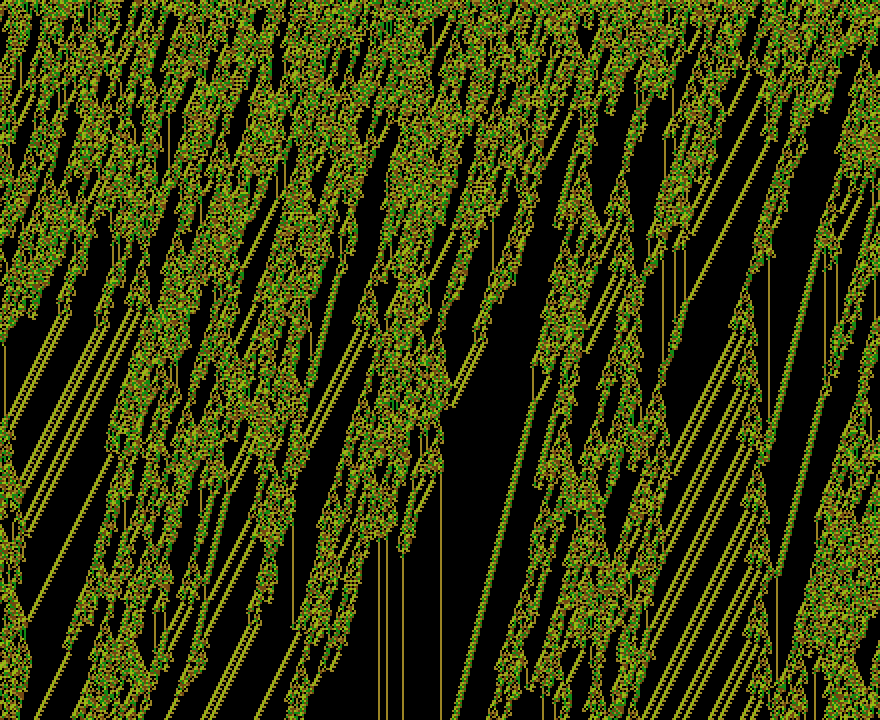
\includegraphics[width=\linewidth]{Class4CA}
\end{center}
\caption{A 5-color cellular automaton with a class 4 rule}
\end{figure}

If you shuffle through enough rules you will almost certainly see all four classes, but I have saved some examples of each kind in the folder \textit{Four\_Classes}.
I noticed that the higher the number of colors, the more likely you are to get class 3 chaotic behavior.
With five colors most of the randomly generated rules are class 3, which is why I limited the number of possible colors to five.
The stable structures of class 2 can also be moving structures which appear as diagonal patterns as in \textit{class2\_example2.npy}.
Classes 3 and 4 appear even with only two colors (see \textit{class3\_example1.npy} and \textit{class4\_example3.npy}).
Some class 4 CA's will have localized structures that tend to die off eventually, as in \textit{class4\_example3.npy}, while others have structures that seem to go on indefinitely.
Sometimes this is related to how fast the localized structures spread out and how fast they die off.
\textit{Fluctuating.npy} is a class 4 rule that both spreads out quickly and dies off quickly, which makes for structures that can last for an unpredictable length of time (also see \textit{Spawn.npy} for an interesting example).
The regions surrounding class 4 structures is often composed of stable structures but can also be chaotic, as in \textit{Chaotic\_environment.npy}.
The boundary between the localized structures and their surroundings can sometimes be unclear (see \textit{Crisscross.npy}).

Not all cellular automaton rules fall neatly into one of the four classes.
\textit{Almost\_stable.npy} is class 3 but has stable structures that can last for a significant time.
Some rules lie somewhere between classes 4 and 3, where the localized structures become packed close together as in  \textit{Class4\_compact1.npy} and \textit{Class4\_compact2.npy}.
See \textit{Hybrid.npy} for an example that contains features of classes 2, 3, and 4.
Sometimes a CA develops separate regions that behave like different classes.
For example, see \textit{Chaotic\_regions.npy}.
In \textit{Binary\_class.npy} the long-term behavior is uncertain:  it can either become all class 3 or all class 2.

An interesting thing to note about classes 3 and 4 is that their randomness does not come from the randomness of their initial condition.
They can often start with a single cell of a different color and get similar long-term behavior.
However, in many cases a certain degree of randomness in the initial condition is required for complex behavior.
You can see this by setting the initial condition to one or five cells with a class 3 or 4 rule and generating random initial conditions.
Sometimes the initial condition can affect the long-term behavior (try observing the long-term behavior of \textit{class3\_example3.npy} with different initial conditions).

It is quite remarkable that such interesting behavior can result from such simple systems.  There is much more to be learned about cellular automata.
\end{document}